\section{Ferramentas de Monorepo}

É necessário desenvolver uma ferramenta tão complexa quanto a da Google para poder implementar a arquitetura de Monorepos? Não, existem diversas ferramentas para construir e gerenciar Monorepos, dentro do ecossistema de Javascript/TypeScript algumas das ferramentas com maior índice de satisfação são: 

\begin{figure}[t]
  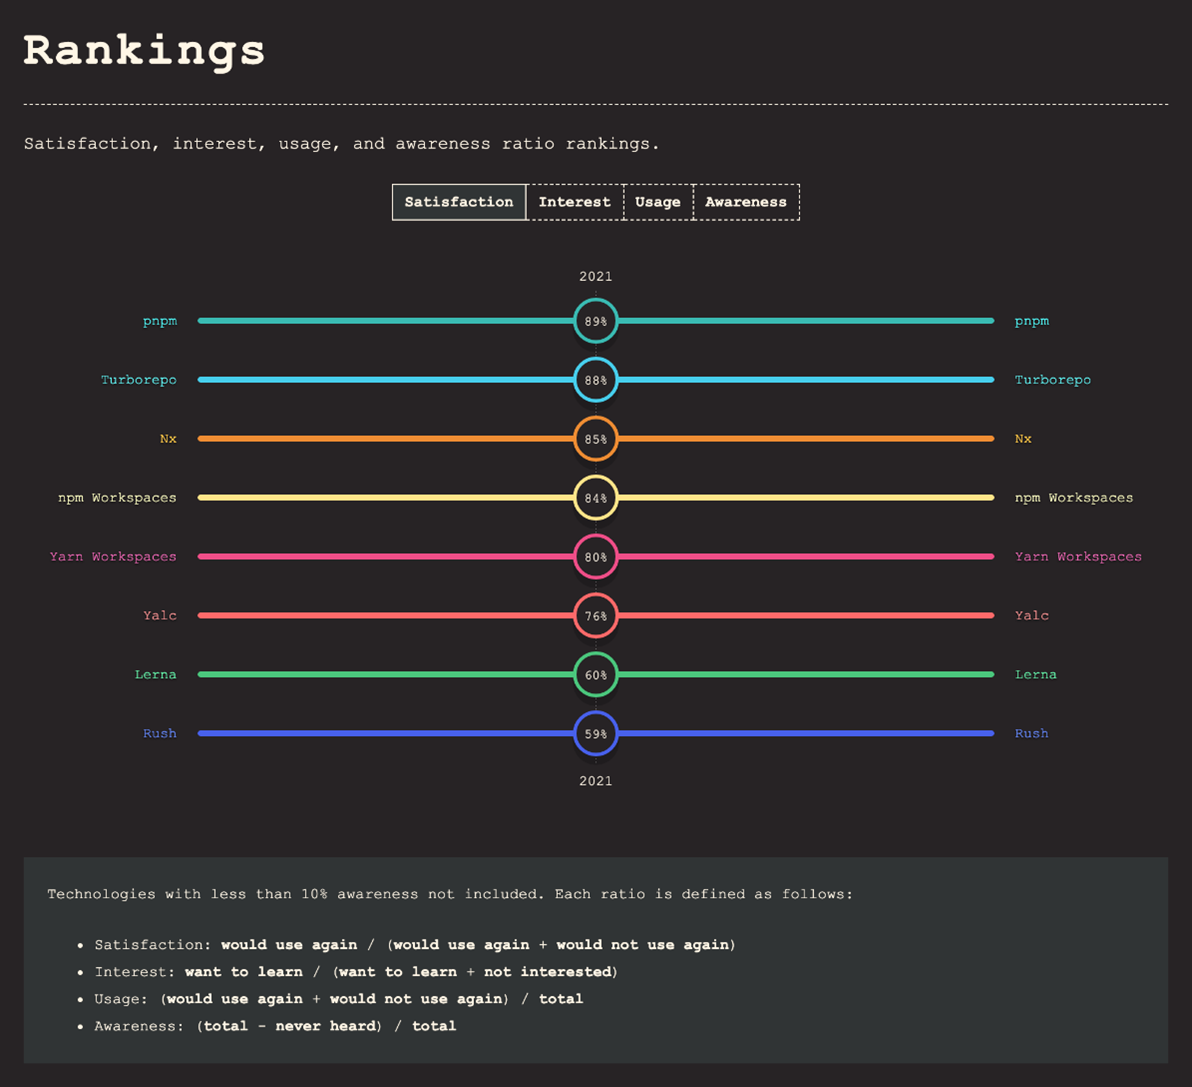
\includegraphics{monorepo-tools.png}
  \centering
  \caption{https://2021.stateofjs.com/en-US/libraries/monorepo-tools}
\end{figure}

Dentre essas ferramentas, uma que vem chamando bastante atenção recentemente é o Turborepo, uma ferramenta desenvolvida por Jared Palmer e que foi adquirida pela empresa Vercel em 2021, e possui diversas funcionalidades para facilitar o gerenciamento de Monorepos além de disponibilizar um registry para salvar o cache de builds de aplicações e pacotes, sendo o complemento ideal para o desenvolvimento de Monorepos rápidos com containers.

O Turborepo é um sistema para gerenciamento de Monorepos em ambientes Javascript e TypeScript, sendo altamente performático, possui diversas ferramentas para alavancar o desenvolvimento com a arquitetura de Monorepos, como por exemplo execuções paralelas, cache em cloud, processos de build incrementais, pipelines para execuções de tarefas, entre outras.
